% section3
\chapter {Determinants}

\section{Determinants; cofactor Expansion}

\begin{exer}
Compute the determinants of the matrix A:
\begin{equation*}
A=\begin{bmatrix}-4 & 1 & 1 & 1 & 1 & \\ 1 & -4 & 1 & 1 & 1 \\ 1 & 1 & -4 & 1 & 1 \\ 1 & 1 & 1 & -4 & 1 \\ 1 & 1 & 1 & 1 & -4\end{bmatrix}\\.
\end{equation*}
How can you construct $A$ brilliantly?
\end{exer}

\begin{sol}

\begin{verbatim}

A=ones(5)-5*eye(5);
disp('A is'); disp(A);
disp('Determinant of A is'); disp(det(A));
\end{verbatim}

\begin{outputs}
\begin{verbatim}

A is
    -4     1     1     1     1
     1    -4     1     1     1
     1     1    -4     1     1
     1     1     1    -4     1
     1     1     1     1    -4

Determinant of A is
  -5.5511e-14
\end{verbatim}
\end{outputs}
\end{sol}

\vspace{3mm}

\begin{exer}
Show that 
$$\det\left(\begin{bmatrix} \displaystyle a & b & c & d \\ -b & a & d & -c \\ -c & -d & a & b \\ -d & c & -b & a \end{bmatrix}\right)=(a^2+b^2+c^2+d^2)^2.$$
\end{exer}

\begin{sol}

\begin{verbatim}

syms a b c d;

A=[a b c d; -b a d -c; -c -d a b; -d c -b a];

disp('Given matrix is'); disp(A);
disp('Determinant of the given matrix is'); 
disp(simplify(det(A)));
\end{verbatim}

\begin{outputs}
\begin{verbatim}

Given matrix is
[  a,  b,  c,  d]
[ -b,  a,  d, -c]
[ -c, -d,  a,  b]
[ -d,  c, -b,  a]
 
Determinant of the given matrix is
(a^2 + b^2 + c^2 + d^2)^2
\end{verbatim}
\end{outputs}
\end{sol}

\vspace{3mm}


\begin{exer} 
The $n$th-order \textbf{Fibonacci matrix} [named for the Italian mathematician~(circa~1170~-~1250)] is the $n \times n$ matrix $F_{n}$ that has 1's on the main diagonal, 1's along the diagonal immediately above the main diagonal, -1's along the diagonal immediately below the main diagonal, and zeros everywhere else. Construct the sequence
$$\det(F_{1}), \,\det(F_{2}), \,\det(F_{3}), \,\cdots, \det(F_{7}).$$
Make a conjecture about the relationship between a term in the sequence and its two immediate predecessors, and then use your conjecture to make a guess at $\det(F_{8})$. Check your guess by calculating this number.
\end{exer}

\begin{sol}
\begin{verbatim}

% Construct the 10x10 Fibonacci matrix F.
N=10; nOnes=ones(N, 1);
F=diag(nOnes)+diag(nOnes(1:N-1),1)-diag(nOnes(1:N-1),-1);

for n=1:7 % n is from 1 to 7
    Fn=F(1:n,1:n); % nxn Fibonacci matrix is selected from F. 
    disp(det(Fn));
end
\end{verbatim}

\begin{outputs}
\begin{verbatim}

     1
     2
     3
     5
     8
    13
    21
\end{verbatim}
\end{outputs}

\noindent The constructed sequence satisfies the relationship $\det(F_n)=\det(F_{n-1})+\det(F_{n-2}),$ for $\det(F_1)=1$ and $\det(F_2)=2$. From that, we may guess that $\det(F_8)=34$.
MATLAB gives us the same output value 34 as our guess. 
\end{sol}

\vspace{3mm}


\begin{exer} Let $A_{n}$ be the $n \times n$ matrix that has 2's along the main diagonal, 1's along the diagonals immediately above and below the main diagonal, and zeros everywhere else. Make a conjecture about the relationship between $n$ and $\det(A_{n})$.
\end{exer}



\begin{sol}
\begin{verbatim}

format rat;
% Construct the 10x10 matrix A satisfying given conditions.
n=10; nOnes=ones(n, 1);
A=2*diag(nOnes)+diag(nOnes(1:n-1),1)+diag(nOnes(1:n-1),-1);

for i=1:10 % i is from 1 to 10
    Ai=A(1:i,1:i); % A_i matrix is selected from A. 
    disp(det(Ai));
end
\end{verbatim}

\begin{outputs}
\begin{verbatim}

       2     
       3       
       4       
       5       
       6       
       7       
       8       
       9       
      10       
      11  
\end{verbatim}
\end{outputs}


\noindent From the outputs, we make a conjecture about the relationship between $n$ and $\det(A_{n})$ as follows:
$$\det(A_{n})=n+1.$$

\end{sol}


\section{Properties of Determinants}

\begin{exer}(\textit{Determinants with LU-decomposition})
In this problem, we find the determinant of the matrix $A$ by using the $LU$-decomposition of $A$, where

\begin{displaymath}
A = \left[\begin{array}{rrrr} -2& \hspace{1mm} 2& \hspace{1mm}-4& \hspace{2mm} -6\\ -3 & 6 & 3 & -15 \\ 5 & -8 & -1 & 17 \\ 1 & 1 & 11 & 7 \end{array} \right].
\end{displaymath}
\vspace{1mm}
\begin{enumerate}
\item[(a)] Compute the determinant of $A$ directly by using the MATLAB command \textit{det} for $A$.
\vspace{1mm}
\item[(b)] Compute the determinant of $A$ by using the MATLAB command \textit{lu} for $A$. Confirm that you get the same results.
\end{enumerate}

\end{exer}


\begin{sol}

\begin{verbatim}

%(a)
A = [-2 2 -4 -6; -3 6 3 -15; 5 -8 -1 17; 1 1 11 7];

det_A = det(A); % Find the determinant of A by using the command det.

disp('The determinant of A by direct use of the command det is');
disp(det_A);

%(b)
[L U P] = lu(A); % We have a PLU-decomposition of A. (i.e., PA=LU ).

% Since the determinant of a triangular matrix is
% just a product of diagonal entries,

det_L = prod(diag(L)); % The product of diagonal entries of L.
% Or, you may use the command det for L, directly. (i.e., det_L = det(L)).

det_U = prod(diag(U)); % The product of diagonal entries of U.
% Or, you may use the command det for U, directly. (i.e., det_U = det(U)).

% If you observe the permutation matrix P, you can see that
% P is an odd permutation. Thus, we have det(P) = -1.
det_P = -1;
% Or, you may use the command det for P, directly. (i.e., det_P = det(P)).

% Since PA = LU, det(P)*det(A) = det(L)*det(U).
det_A = det_P * det_L * det_U;

disp('The determinant of A by using the LU-decomposition is'); disp(det_A);
\end{verbatim}


\begin{outputs}

\begin{verbatim}

The determinant of A by direct use of the command det is
   24.0000

The determinant of A by using the PLU-decomposition is
   24.0000
\end{verbatim}

\end{outputs}

\end{sol}
 
\vspace{3mm}

\begin{exer} (\textit{Effects of Elementary Row Operations on the Determinant})

Using the MATLAB command \textit{det}, confirm the formulas (a)-(c) in Theorem 4.2.2 of Section 4.2 for the matrix $A$ given in the problem 31 of Exercise set 4.1.
\end{exer}

\begin{sol}
\begin{verbatim}

A = [3 3 0 5; 2 2 0 -2; 4 1 -3 0; 2 10 3 2];

% (a). Multiply the second row of A by 2 and call it A2.
% Initialize the matrix A2 as A.
A2 = A; 
% Multiply the second row of A by 2.
A2(2,:) = 2*A(2,:);
disp('The determinant of A2 is'); disp(det(A2));
disp('2*det(A) = '); disp(2*det(A));

% (b). Interchange the rows 2 and 4 of A and call it A24.
% Initialize the matrix A24 as A.
A24 = A; 
% Interchange the rows 2 and 4 of A.
A24(2, :) = A(4, :) ; A24(4, :) = A(2, :);
disp('The determinant of A24 is'); disp(det(A24));
disp('-det(A) = '); disp(-det(A));

% (c). Add 2 times row 3 to row 4 of A and call it A234.
% Initialize the matrix A234 as A.
A234 = A; 
% Add 2 times row 3 of A to row 4.
A234(4, :) = 2 * A(3, :) + A(4, :); 
disp('The determinant of A234 is'); disp(det(A234));
disp('det(A) = '); disp(det(A));
\end{verbatim}

\begin{outputs}

\begin{verbatim}

The determinant of A2 is
  -480
2*det(A) =
 -480.0000

The determinant of A24 is
  240.0000
-det(A) =
  240.0000

The determinant of A234 is
 -240.0000
det(A) =
 -240.0000
\end{verbatim}
\end{outputs}
\end{sol}


\vspace{3mm}

\begin{exer} Use a determinant to show that if $a, b, c,$ and $d$ are not all zeros, then the vectors
\begin{eqnarray*}
\mathbf{v}_{1}&=&(a,\, b,\, c,\, d)\\
\mathbf{v}_{2}&=&(-b, a, d, -c)\\
\mathbf{v}_{3}&=&(-c, -d, a, b)\\
\mathbf{v}_{4}&=&(-d, c, -b, a)
\end{eqnarray*}
are linearly independent.
\end{exer}

\begin{sol}

\begin{verbatim}

syms a b c d;
v1=[a b c d];
v2=[-b a d -c];
v3=[-c -d a b];
v4=[-d c -b a];

V=[v1; v2; v3; v4];
disp('det(V) is'); disp(simplify(det(V)));
\end{verbatim}

\begin{outputs}
\begin{verbatim}

det(V) is
(a^2 + b^2 + c^2 + d^2)^2
\end{verbatim}

\end{outputs}

\end{sol}


\section{Cramer's Rule; Formula for $A^{-1}$; Applications}

No MATLAB problems in this section.

\newpage

\section{A First Look at Eigenvalues and Eigenvectors}


\begin{exer}(\textit{Eigenvalues and Eigenvectors})\\
Use the MATLAB command \textit{eig} to find the eigenvalues and the associated \mbox{eigenvectors} of the matrix $A$, where
$$A = \left[\begin{array}{rrrr} 2& \hspace{1mm}-3& \hspace{1mm} 1& \hspace{3mm} 0\\ 1 & 1 & 2 & 2\\ 3 & 0 & -1 & 4 \\ 1 & 6 & 5 & 6 \end{array} \right].$$
Display the results with long digits.
\end{exer}

\begin{sol}

\begin{verbatim}

% Construct the matrix A.
A=[2 -3 1 0; 1 1 2 2; 3 0 -1 4; 1 6 5 6];

% Find the eigenvalues and eigenvectors of A by using eig.
% This command gives AQ = QD.
[Q D] = eig(A); 
lambda1 = D(1,1); lambda2 = D(2,2); 
lambda3 = D(3,3); lambda4 = D(4,4); 

% Extract each column vector as an eigenvector of A.
x1 = Q(:,1); x2 = Q(:,2); x3 = Q(:,3); x4 = Q(:,4);

% Display the result with long digits.
format long; 
disp('lambda1 is'); disp(lambda1);
disp('The eigenvector corresponding to lambda1 is'); disp(x1');
disp('lambda2 is'); disp(lambda2);
disp('The eigenvector corresponding to lambda2 is'); disp(x2');
disp('lambda3 is'); disp(lambda3);
disp('The eigenvector corresponding to lambda3 is'); disp(x3');
disp('lambda4 is'); disp(lambda4);
disp('The eigenvector corresponding to lambda4 is'); disp(x4');
\end{verbatim}

\begin{outputs}
\begin{verbatim}

lambda1 is
  9.561855032395805
The eigenvector corresponding to lambda1 is
 -0.067716707308095  0.278176502030497  0.322465582156500  0.902246213399589
lambda2 is
 -3.364648937746373
The eigenvector corresponding to lambda2 is
  0.275562522991092  0.197508356444458 -0.885771126913498  0.316962546342283
lambda3 is
  1.802793905350564
The eigenvector corresponding to lambda3 is
 -0.833621905475750 -0.103812731179200 -0.147042873144503  0.522183711938150
lambda4 is
 -3.860931435448914e-16
The eigenvector corresponding to lambda4 is
 -0.705886578756789 -0.456750139195570  0.041522739926871  0.539795619049310
\end{verbatim}

\end{outputs}


\noindent\textit{Remark.} In fact, if we compute $\lambda_{4}$ by hand, we can obtain that $\lambda_{4}=0$. However, from the result, we see that the resulting value of $\lambda_{4}$ seems to be nonzero even though it is small enough. This is due to roundoff errors in arithmetic operations. Please refer to the help command of \textit{eps}, then you can see that $eps = 2.220446049250313e-016$ is floating-point relative accuracy, which means that \textit{eps} value is the allowable tolerance when we do numerical computations with rounding floating-point number off. ($i.e.$, $eps$ is an upper bound on the relative error due to rounding in floating point arithmetic.)
Therefore, we can regard the resulting value of $\lambda_{4}$ as zero.
\end{sol}

\vspace{3mm}

\begin{exer}(\textit{Eigenvalues and Eigenvectors})

Define an $n$th-order \textbf\textit{checkboard matrix} $C_{n}$ to be a matrix that has a 1 in the upper left corner and alternates between 1 and 0 along rows and columns (see the figure below). Find the eigenvalues of $C_{1}, C_{2}, \cdots$ to make a conjecture about the eigenvalues of $C_{n}$. What can you say about the eigenvalues of $C_{n}$? 
\begin{figure}[h]\centering
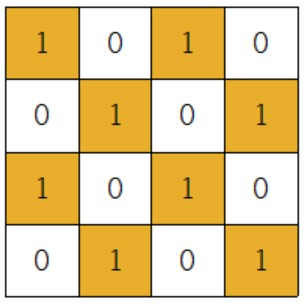
\includegraphics[width=4cm]{figure.jpg}
\end{figure}
\end{exer}

\begin{sol}
\begin{verbatim}

format short;
n=10;   % Set the size of the large check board

% Construct your checkboard
CheckBoard=zeros(n);    
CheckBoard(1:2:n, 1:2:n)=1;
CheckBoard(2:2:n, 2:2:n)=1;
for i=1:n
    Cn=CheckBoard(1:i, 1:i);
    [Qn Dn]=eig(Cn);    % Eigenvectors and eigenvalues
    fprintf('The size of the checkboard is %d \n',i);
    disp(diag(Dn)');
end
\end{verbatim}

\begin{outputs}

\begin{verbatim}

The size of the checkboard is 1 
     1
The size of the checkboard is 2 
     1 1
The size of the checkboard is 3 
     0 1 2
The size of the checkboard is 4 
     0 0 2 2
The size of the checkboard is 5 
   -0.0000 -0.0000  0.0000  2.0000  3.0000
The size of the checkboard is 6 
   -0.0000  -0.0000  -0.0000  -0.0000  3.0000  3.0000
The size of the checkboard is 7 
   -0.0000  -0.0000   0.0000   0.0000  0.0000  3.0000  4.0000
The size of the checkboard is 8 
   -0.0000  -0.0000  -0.0000  0.0000  0.0000  0.0000  4.0000  4.0000
The size of the checkboard is 9 
   -0.0000  -0.0000  -0.0000 -0.0000   0   0.0000  0.0000  4.0000  5.0000
The size of the checkboard is 10 
   -0.0000  -0.0000  -0.0000  0  0.0000  0.0000  0.0000  0.0000  5.0000  5.0000
\end{verbatim}
\end{outputs}


\noindent We may conclude that the eigenvalues of $C_{n}$ are given as follows:
$$\begin{cases} 1 &\text{if $n=1$,}\\ 
 k,\, k,\, \underbrace{0,\,0,\,\cdots,\,0}_{(n-2)}&\text{if $n=2k$,}\\
 k,\,k+1,\,\underbrace{0,\,0,\,\cdots,\,0}_{(n-2)}&\text{if $n=2k+1$,}
\end{cases}
$$ 
where $k$ is a positive integer.
\end{sol}
